%**************************************************************************************
% SINDy: Sparse Identification of Nonlinear Dynamics
% License: CC BY-NC-SA 4.0 (http://creativecommons.org/licenses/by-nc-sa/4.0/)
%**************************************************************************************

\documentclass{beamer}

\mode<presentation> {
\usetheme{Madrid}

% Burnt orange
\definecolor{burntorange}{rgb}{0.8, 0.33, 0.0}
\colorlet{beamer@blendedblue}{burntorange}
% Pale yellow
\definecolor{paleyellow}{rgb}{1.0, 1.0, 0.953}
\setbeamercolor{background canvas}{bg=paleyellow}
% Secondary and tertiary palette
\setbeamercolor*{palette secondary}{use=structure,fg=white,bg=burntorange!80!black}
\setbeamercolor*{palette tertiary}{use=structure,fg=white,bg=burntorange!60!black}
}

\usepackage{amsmath}
\usepackage{amssymb}
\DeclareMathOperator*{\argmin}{arg\,min}
\DeclareMathOperator*{\argmax}{arg\,max}
\usepackage{bm}
\usepackage{booktabs}
\usepackage{graphicx}
\usepackage{xcolor}
\usepackage{tikz}
\usetikzlibrary{positioning,calc,shapes.geometric,arrows.meta}

%----------------------------------------------------------------------------------------
%	TITLE PAGE
%----------------------------------------------------------------------------------------

\title[SINDy]{Sparse Identification of Nonlinear Dynamics (SINDy)}

\author{Krishna Kumar}
\institute[UT Austin]{
University of Texas at Austin
}
\date{\today}

\begin{document}

\begin{frame}
\titlepage
\end{frame}

%----------------------------------------------------------------------------------------
\begin{frame}
\frametitle{Overview}
\tableofcontents
\end{frame}

%========================================================================================
\section{Introduction}
%========================================================================================

%----------------------------------------------------------------------------------------
\begin{frame}
\frametitle{The Discovery Problem}

\textbf{Traditional Approach:}
\begin{itemize}
\item Scientist observes system behavior
\item Proposes governing equations based on physical intuition
\item Validates through experiments
\end{itemize}

\vspace{0.5cm}

\textbf{Modern Challenge:}
\begin{itemize}
\item Complex systems: climate, turbulence, biological networks
\item High-dimensional data available
\item Governing equations unknown or intractable
\end{itemize}

\vspace{0.5cm}

\textbf{The Question:}

\begin{center}
\Large
Can we discover governing equations directly from data?
\end{center}

\end{frame}

%----------------------------------------------------------------------------------------
\begin{frame}
\frametitle{What is SINDy?}

\textbf{Sparse Identification of Nonlinear Dynamics}

\vspace{0.3cm}

Given measurements $\mathbf{u}(t) \in \mathbb{R}^n$ from a physical system, discover:

\begin{equation}
\frac{d\mathbf{u}}{dt} = \mathbf{f}(\mathbf{u})
\end{equation}

\vspace{0.3cm}

\textbf{Key Insights:}
\begin{enumerate}
\item Most physical systems have \textbf{sparse} dynamics (few active terms)
\item $\mathbf{f}$ can be represented as a linear combination of basis functions
\item Use sparse regression to identify the active terms
\end{enumerate}

\vspace{0.3cm}

\textbf{Why Sparsity?}
\begin{itemize}
\item Occam's Razor: simplest explanation is often correct
\item Physical laws typically involve few terms
\item Example: $F = ma$, not $F = ma + 0 \cdot v^2 + 0 \cdot a^3 + \ldots$
\end{itemize}

\end{frame}

%----------------------------------------------------------------------------------------
\begin{frame}
\frametitle{Example: Lorenz System}

The Lorenz equations (unknown to us):
\begin{align*}
\dot{x} &= \sigma(y - x) \\
\dot{y} &= x(\rho - z) - y \\
\dot{z} &= xy - \beta z
\end{align*}

\vspace{0.3cm}

\textbf{What we have:} Time series data $\{(x_i, y_i, z_i, t_i)\}_{i=1}^m$

\vspace{0.3cm}

\textbf{What we want:} The equations above!

\vspace{0.3cm}

\textbf{Key observation:} Each equation is sparse in polynomial space
\begin{itemize}
\item Only 2-3 terms out of many possible polynomials
\item Example: $\dot{x}$ only involves $x, y$ (not $x^2, xy^2, \ldots$)
\end{itemize}

\end{frame}

%========================================================================================
\section{How SINDy Works: An Explanation}
%========================================================================================

%----------------------------------------------------------------------------------------
\begin{frame}
\frametitle{What is SINDy?}

SINDy = \textbf{Sparse Identification of Nonlinear Dynamics}

\vspace{0.5cm}

\textbf{The big idea:} Discover governing equations just by looking at data.

\vspace{0.5cm}

\textbf{Example scenario:}
\begin{itemize}
\item Watch a pendulum swing
\item Record position and velocity at different times
\item Don't know any physics ($F=ma$, gravity, etc.)
\item SINDy analyzes the data and tells you the exact differential equation
\end{itemize}

\vspace{0.5cm}

\textbf{Output:}
$$\frac{d^2\theta}{dt^2} = -\frac{g}{L} \sin(\theta)$$

\end{frame}

%----------------------------------------------------------------------------------------
\begin{frame}
\frametitle{The Core Assumption: Physics is Sparse}

Most physical systems are governed by equations with \textbf{only a few important terms}.

\vspace{0.5cm}

\textbf{Example:} Simple pendulum
$$\frac{d^2\theta}{dt^2} = -\frac{g}{L} \sin(\theta)$$

\vspace{0.3cm}

We could try thousands of mathematical terms:
\begin{itemize}
\item Polynomials: $\theta^2, \theta^3, \theta^4, \ldots$
\item Trig functions: $\cos(\theta), \tan(\theta), \sin^2(\theta), \ldots$
\item Exponentials: $e^\theta, e^{-\theta}, \ldots$
\end{itemize}

\vspace{0.3cm}

But the true equation uses only \textbf{one}: $\sin(\theta)$

\vspace{0.3cm}

\textbf{Sparsity:} The governing equation is simple among a sea of possibilities.

\end{frame}

%----------------------------------------------------------------------------------------
\begin{frame}
\frametitle{Step-by-Step Guide: Step 1}
\framesubtitle{Collect Data (and Get Derivatives)}

\textbf{What you need:}
\begin{enumerate}
\item State of your system over time
\begin{itemize}
\item For pendulum: angle $\theta$ and angular velocity $\omega$
\item Measured at many time points $t$
\end{itemize}

\item Time derivatives $\dot{X}$ (how fast each variable changes)
\begin{itemize}
\item Sometimes measured directly (e.g., accelerometer)
\item Often calculated numerically from data (slope between nearby points)
\end{itemize}
\end{enumerate}

\vspace{0.5cm}

\textbf{Result:} Two data matrices
\begin{itemize}
\item $X$: State at all times (e.g., $[\theta, \omega]$)
\item $\dot{X}$: Rate of change at all times (e.g., $[\dot{\theta}, \dot{\omega}]$)
\end{itemize}

\end{frame}

%----------------------------------------------------------------------------------------
\begin{frame}
\frametitle{Step-by-Step Guide: Step 2}
\framesubtitle{Build a Library of Candidate Functions}

SINDy doesn't know if the answer involves $x^2$, $\sin(x)$, or $xy$.

\vspace{0.3cm}

\textbf{Solution:} Propose a huge library $\Theta$ of all candidate functions.

\vspace{0.5cm}

\textbf{Example:} If state variables are $x, y$, library might include:

\begin{columns}[T]
\column{0.45\textwidth}
\begin{itemize}
\item Constants: $1$
\item Linear: $x, y$
\item Quadratic: $x^2, y^2, xy$
\item Cubic: $x^3, x^2y, xy^2, y^3$
\end{itemize}

\column{0.45\textwidth}
\begin{itemize}
\item Trig: $\sin(x), \cos(x), \sin(y), \cos(y)$
\item Other: $1/x, e^x, \log(y)$
\end{itemize}
\end{columns}

\vspace{0.5cm}

\textbf{Result:} Matrix $\Theta(X)$ where each column is one function evaluated at every time step.

\end{frame}

%----------------------------------------------------------------------------------------
\begin{frame}
\frametitle{Step-by-Step Guide: Step 3}
\framesubtitle{Set Up "Find the Coefficients" Problem}

SINDy finds a combination of library functions that equals your derivative.

\vspace{0.5cm}

\textbf{Linear algebra problem:}
$$\dot{X} \approx \Theta(X) \cdot \Xi$$

\begin{itemize}
\item $\dot{X}$ = Time derivatives (what you want to explain)
\item $\Theta(X)$ = Library of candidate functions (building blocks)
\item $\Xi$ (Xi) = Unknown coefficients (what you need to find)
\end{itemize}

\vspace{0.5cm}

\textbf{For system with $x, y$:}
\begin{align*}
\dot{x} &= c_1(1) + c_2(x) + c_3(y) + c_4(x^2) + c_5(xy) + \ldots \\
\dot{y} &= d_1(1) + d_2(x) + d_3(y) + d_4(x^2) + d_5(xy) + \ldots
\end{align*}

\textbf{Goal:} Find all coefficients $(c_i, d_i)$.

\end{frame}

%----------------------------------------------------------------------------------------
\begin{frame}
\frametitle{Step-by-Step Guide: Step 4}
\framesubtitle{Find the Sparse Solution (The Magic)}

Standard least-squares regression would find a solution, but:
\begin{itemize}
\item Uses all library functions a little bit
\item Tiny non-zero values for every coefficient
\item Accurate but impossible to interpret
\end{itemize}

\vspace{0.5cm}

\textbf{SINDy's trick: Sparse regression}

Instead of most accurate, find \textbf{simplest solution that is still highly accurate}.

\vspace{0.3cm}

Force as many coefficients $\Xi$ as possible to be \textbf{exactly zero}.

\vspace{0.5cm}

\textbf{Algorithm: Sequentially Thresholded Least Squares (STLSQ)}
\begin{enumerate}
\item Solve for all coefficients
\item Find coefficients below threshold
\item Set small coefficients to zero permanently
\item Re-solve with only remaining "active" coefficients
\item Repeat until stable
\end{enumerate}

\end{frame}

%----------------------------------------------------------------------------------------
\begin{frame}
\frametitle{The Final Result}

After sparse regression, $\Xi$ matrix is mostly zeros.

\vspace{0.3cm}

The few non-zero entries tell you \textbf{exactly which terms} build the governing equation.

\vspace{0.5cm}

\textbf{Example: Chaotic Lorenz system}

Variables: $x, y, z$

\vspace{0.3cm}

\textbf{SINDy discovers from data alone:}
\begin{align*}
\dot{x} &= -10x + 10y \\
\dot{y} &= 28x - y - xz \\
\dot{z} &= -\frac{8}{3}z + xy
\end{align*}

\vspace{0.3cm}

Found by identifying non-zero coefficients for terms: $x, y, xz, z, xy$

\vspace{0.3cm}

\textbf{Key insight:} Turns messy data into simple, interpretable differential equations.

\end{frame}

%========================================================================================
\section{Mathematical Framework}
%========================================================================================

%----------------------------------------------------------------------------------------
\begin{frame}
\frametitle{The SINDy Equation}

\textbf{Core approximation problem:}

\begin{equation}
\dot{\mathbf{U}} \approx \boldsymbol{\Theta}(\mathbf{U})\boldsymbol{\Xi}
\end{equation}

\vspace{0.5cm}

\begin{columns}[T]

\column{0.3\textwidth}
\textbf{Data Matrix}
$$\mathbf{U} = \begin{bmatrix}
u_1(t_1) & \cdots & u_n(t_1) \\
u_1(t_2) & \cdots & u_n(t_2) \\
\vdots & & \vdots \\
u_1(t_m) & \cdots & u_n(t_m)
\end{bmatrix}$$
$m$ samples\\
$n$ states

\column{0.3\textwidth}
\textbf{Library Matrix}
$$\boldsymbol{\Theta}(\mathbf{U}) = \begin{bmatrix}
\mid & & \mid \\
\theta_1(\mathbf{U}) & \cdots & \theta_\ell(\mathbf{U}) \\
\mid & & \mid
\end{bmatrix}$$
$\ell$ candidate\\
functions

\column{0.3\textwidth}
\textbf{Coefficients}
$$\boldsymbol{\Xi} = \begin{bmatrix}
\mid & & \mid \\
\xi_1 & \cdots & \xi_n \\
\mid & & \mid
\end{bmatrix}$$
Sparse!\\
\phantom{x}

\end{columns}

\vspace{0.5cm}

\textbf{Goal:} Find sparse $\boldsymbol{\Xi}$ such that $\boldsymbol{\Theta}(\mathbf{U})\boldsymbol{\Xi} \approx \dot{\mathbf{U}}$

\end{frame}

%----------------------------------------------------------------------------------------
\begin{frame}
\frametitle{Data Matrix $\mathbf{U}$}

Collect measurements at $m$ time points:

$$\mathbf{U} = \begin{bmatrix}
u_1(t_1) & u_2(t_1) & \cdots & u_n(t_1) \\
u_1(t_2) & u_2(t_2) & \cdots & u_n(t_2) \\
\vdots & \vdots & & \vdots \\
u_1(t_m) & u_2(t_m) & \cdots & u_n(t_m)
\end{bmatrix}_{m \times n}$$

\vspace{0.3cm}

\textbf{Derivatives:} Compute numerically or measure directly

$$\dot{\mathbf{U}} = \begin{bmatrix}
\dot{u}_1(t_1) & \dot{u}_2(t_1) & \cdots & \dot{u}_n(t_1) \\
\dot{u}_1(t_2) & \dot{u}_2(t_2) & \cdots & \dot{u}_n(t_2) \\
\vdots & \vdots & & \vdots \\
\dot{u}_1(t_m) & \dot{u}_2(t_m) & \cdots & \dot{u}_n(t_m)
\end{bmatrix}_{m \times n}$$

\vspace{0.3cm}

\textbf{Methods for computing $\dot{\mathbf{U}}$:}
\begin{itemize}
\item Finite differences: simple but noisy
\item Total variation regularization: noise-robust
\item Polynomial interpolation + differentiation
\end{itemize}

\end{frame}

%----------------------------------------------------------------------------------------
\begin{frame}
\frametitle{Library Matrix $\boldsymbol{\Theta}(\mathbf{U})$}

Build library of candidate functions applied to data:

$$\boldsymbol{\Theta}(\mathbf{U}) = \begin{bmatrix}
1 & u_1 & u_2 & \cdots & u_n & u_1^2 & u_1u_2 & \cdots
\end{bmatrix}$$

\vspace{0.3cm}

\textbf{Polynomial Library (degree $d$):}
\begin{itemize}
\item Constant: $1$
\item Linear: $u_1, u_2, \ldots, u_n$
\item Quadratic: $u_1^2, u_1u_2, u_1u_3, \ldots, u_n^2$
\item Cubic: $u_1^3, u_1^2u_2, \ldots, u_n^3$
\item $\vdots$
\end{itemize}

\vspace{0.3cm}

\textbf{Other Options:}
\begin{itemize}
\item Trigonometric: $\sin(u_i), \cos(u_i)$
\item Exponential: $e^{u_i}$
\item Rational: $\frac{1}{u_i}$
\item Custom: domain-specific functions
\end{itemize}

\end{frame}

%----------------------------------------------------------------------------------------
\begin{frame}
\frametitle{Example: 2D Polynomial Library}

For $\mathbf{u} = [x, y]^T$ with degree 2:

\vspace{0.3cm}

$$\boldsymbol{\Theta}(\mathbf{u}) = \begin{bmatrix}
1 & x & y & x^2 & xy & y^2
\end{bmatrix}$$

\vspace{0.5cm}

\textbf{For Lorenz system} $(x, y, z)$ with degree 2:

$$\boldsymbol{\Theta}(\mathbf{u}) = \begin{bmatrix}
1 & x & y & z & x^2 & xy & xz & y^2 & yz & z^2
\end{bmatrix}$$

\vspace{0.5cm}

Each row of $\boldsymbol{\Theta}(\mathbf{U})$ evaluates these functions at one time point.

\vspace{0.3cm}

\textbf{Size:} $m \times \ell$ where $\ell$ = number of basis functions

For Lorenz: $\ell = 10$ (1 constant + 3 linear + 6 quadratic)

\end{frame}

%----------------------------------------------------------------------------------------
\begin{frame}
\frametitle{Coefficient Matrix $\boldsymbol{\Xi}$}

Each column $\xi_i$ gives coefficients for the $i$-th state equation:

$$\boldsymbol{\Xi} = \begin{bmatrix}
\xi_{0,1} & \xi_{0,2} & \cdots & \xi_{0,n} \\
\xi_{1,1} & \xi_{1,2} & \cdots & \xi_{1,n} \\
\vdots & \vdots & & \vdots \\
\xi_{\ell,1} & \xi_{\ell,2} & \cdots & \xi_{\ell,n}
\end{bmatrix}_{\ell \times n}$$

\vspace{0.3cm}

\textbf{Interpretation:} The $i$-th dynamical equation is

$$\dot{u}_i = \sum_{j=1}^\ell \xi_{j,i} \theta_j(\mathbf{u})$$

\vspace{0.3cm}

\textbf{Sparsity:} Most entries of $\boldsymbol{\Xi}$ should be zero!

\vspace{0.3cm}

Example: If $\dot{x} = -10x + 10y$, then
$$\xi_{\text{for } \dot{x}} = [0, -10, 10, 0, 0, 0, \ldots, 0]^T$$

\end{frame}

%========================================================================================
\section{The SINDy Algorithm}
%========================================================================================

%----------------------------------------------------------------------------------------
\begin{frame}
\frametitle{Overview of SINDy Algorithm}

\begin{center}
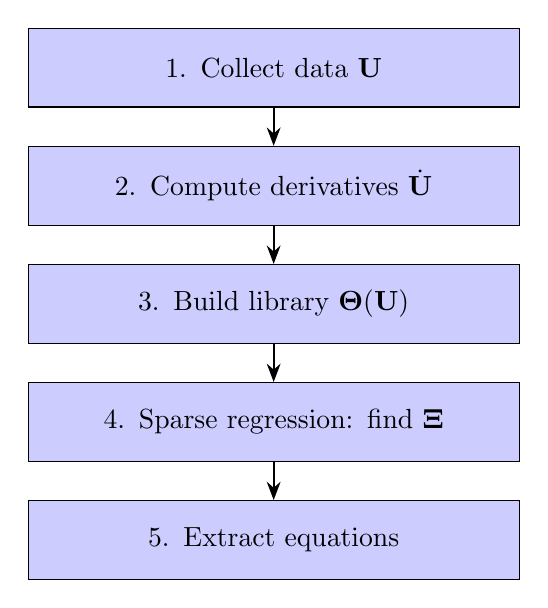
\begin{tikzpicture}[
    box/.style={rectangle, draw, fill=blue!20, text width=6cm, align=center, minimum height=1cm},
    arrow/.style={->, >=Stealth, thick}
]

\node[box] (data) at (0,0) {1. Collect data $\mathbf{U}$};
\node[box] (deriv) at (0,-1.5) {2. Compute derivatives $\dot{\mathbf{U}}$};
\node[box] (library) at (0,-3) {3. Build library $\boldsymbol{\Theta}(\mathbf{U})$};
\node[box] (sparse) at (0,-4.5) {4. Sparse regression: find $\boldsymbol{\Xi}$};
\node[box] (equation) at (0,-6) {5. Extract equations};

\draw[arrow] (data) -- (deriv);
\draw[arrow] (deriv) -- (library);
\draw[arrow] (library) -- (sparse);
\draw[arrow] (sparse) -- (equation);

\end{tikzpicture}
\end{center}

\end{frame}

%----------------------------------------------------------------------------------------
\begin{frame}
\frametitle{Step 1-3: Data Preparation}

\textbf{1. Collect Data}
\begin{itemize}
\item Measure system at times $t_1, t_2, \ldots, t_m$
\item Store in matrix $\mathbf{U}$ (size $m \times n$)
\end{itemize}

\vspace{0.3cm}

\textbf{2. Compute Derivatives}
\begin{itemize}
\item Finite differences: $\dot{u}(t_i) \approx \frac{u(t_{i+1}) - u(t_i)}{\Delta t}$
\item Or use higher-order methods
\item Store in matrix $\dot{\mathbf{U}}$ (size $m \times n$)
\end{itemize}

\vspace{0.3cm}

\textbf{3. Build Library}
\begin{itemize}
\item Choose basis functions: polynomials, trig, etc.
\item Evaluate at each data point
\item Store in matrix $\boldsymbol{\Theta}(\mathbf{U})$ (size $m \times \ell$)
\end{itemize}

\end{frame}

%----------------------------------------------------------------------------------------
\begin{frame}
\frametitle{Step 4: Sparse Regression}

\textbf{Problem:} Solve $\dot{\mathbf{U}} \approx \boldsymbol{\Theta}(\mathbf{U})\boldsymbol{\Xi}$ with sparse $\boldsymbol{\Xi}$

\vspace{0.3cm}

This is $n$ separate sparse regression problems (one per column):

$$\dot{\mathbf{u}}_i \approx \boldsymbol{\Theta}(\mathbf{U})\xi_i \quad \text{for } i = 1, \ldots, n$$

\vspace{0.3cm}

\textbf{Methods:}
\begin{itemize}
\item \textbf{LASSO:} $\min_{\xi} \|\dot{\mathbf{u}} - \boldsymbol{\Theta}\xi\|_2^2 + \lambda \|\xi\|_1$
\item \textbf{Ridge:} $\min_{\xi} \|\dot{\mathbf{u}} - \boldsymbol{\Theta}\xi\|_2^2 + \lambda \|\xi\|_2^2$
\item \textbf{Elastic Net:} Combination of LASSO + Ridge
\item \textbf{STLSQ:} Sequential Thresholded Least Squares (SINDy default)
\end{itemize}

\vspace{0.3cm}

\textbf{Why not plain least squares?}
\begin{itemize}
\item Would give dense solution (all coefficients non-zero)
\item Overfitting and no interpretability
\end{itemize}

\end{frame}

%----------------------------------------------------------------------------------------
\begin{frame}
\frametitle{STLSQ: Sequential Thresholded Least Squares}

\textbf{Algorithm:}

\begin{enumerate}
\item Solve least squares: $\xi \leftarrow \argmin_{\xi} \|\dot{\mathbf{u}} - \boldsymbol{\Theta}\xi\|_2^2$
\item Threshold: Set $\xi_j = 0$ if $|\xi_j| < \lambda$
\item Re-solve using only active terms (non-zero $\xi_j$)
\item Repeat steps 2-3 until convergence
\end{enumerate}

\vspace{0.5cm}

\textbf{Why STLSQ?}
\begin{itemize}
\item Faster than LASSO for large problems
\item More stable numerically
\item Simple and effective
\end{itemize}

\vspace{0.3cm}

\textbf{Key parameter:} Threshold $\lambda$
\begin{itemize}
\item Too small: not sparse enough, overfitting
\item Too large: miss important terms, underfitting
\end{itemize}

\end{frame}

%----------------------------------------------------------------------------------------
\begin{frame}
\frametitle{STLSQ Example}

Consider $\dot{x} = -2x$ with library $[1, x, x^2, x^3]$

\vspace{0.3cm}

\textbf{Iteration 0:} Least squares solution
$$\xi = [0.05, -2.01, -0.03, 0.02]^T$$

\vspace{0.3cm}

\textbf{Iteration 1:} Threshold at $\lambda = 0.1$
$$\xi = [0, -2.01, 0, 0]^T \quad \text{(set small values to 0)}$$

\vspace{0.3cm}

\textbf{Iteration 2:} Re-solve with only $x$ term active
$$\xi = [0, -2.00, 0, 0]^T$$

\vspace{0.3cm}

\textbf{Iteration 3:} Converged! (no change)

\vspace{0.3cm}

\textbf{Discovered equation:} $\dot{x} = -2x$ (exact!)

\end{frame}

%========================================================================================
\section{Examples}
%========================================================================================

%----------------------------------------------------------------------------------------
\begin{frame}
\frametitle{Example 1: Linear System}

\textbf{True system:}
\begin{align*}
\dot{x} &= -2x \\
\dot{y} &= y
\end{align*}

\vspace{0.3cm}

\textbf{Setup:}
\begin{itemize}
\item Initial condition: $(x_0, y_0) = (3, 0.5)$
\item Sample 100 time points over $t \in [0, 1]$
\item Polynomial library with degree 3
\item STLSQ with threshold $\lambda = 0.2$
\end{itemize}

\vspace{0.3cm}

\textbf{SINDy discovers:}
\begin{align*}
\dot{x} &= -2.000x \\
\dot{y} &= 1.000y
\end{align*}

Perfect recovery!

\end{frame}

%----------------------------------------------------------------------------------------
\begin{frame}
\frametitle{Example 2: Lorenz System}

\textbf{True system:} ($\sigma = 10, \rho = 28, \beta = 8/3$)
\begin{align*}
\dot{x} &= 10(y - x) \\
\dot{y} &= x(28 - z) - y = 28x - xz - y \\
\dot{z} &= xy - \frac{8}{3}z
\end{align*}

\vspace{0.3cm}

\textbf{SINDy discovers:} (threshold $\lambda = 0.025$)
\begin{align*}
\dot{x} &= -10.005x + 10.004y \\
\dot{y} &= 27.805x - 0.958y - 0.993xz \\
\dot{z} &= -2.667z + 0.999xy
\end{align*}

\vspace{0.3cm}

Very close! Small errors due to:
\begin{itemize}
\item Numerical differentiation noise
\item Finite data
\end{itemize}

\end{frame}

%----------------------------------------------------------------------------------------
\begin{frame}
\frametitle{Lorenz: Library Comparison}

\textbf{With polynomial library (degree 2):}
\begin{itemize}
\item Sparse, accurate solution
\item Correct terms identified
\end{itemize}

\vspace{0.5cm}

\textbf{With Fourier library (sines and cosines):}
\begin{align*}
\dot{x} &= 0.772\sin(x) + 2.097\cos(x) - 2.298\sin(y) - 3.115\cos(y) \\
\dot{y} &= 1.362\sin(y) - 0.222\cos(y)
\end{align*}

\begin{itemize}
\item Not sparse!
\item Poor approximation
\item Many terms with similar magnitudes
\end{itemize}

\vspace{0.3cm}

\textbf{Lesson:} Library choice matters! Must match system's structure.

\end{frame}

%========================================================================================
\section{Implementation}
%========================================================================================

%----------------------------------------------------------------------------------------
\begin{frame}[fragile]
\frametitle{PySINDy: Python Implementation}

\textbf{Three main components:}

\begin{enumerate}
\item \texttt{pysindy.differentiation}: Compute $\dot{\mathbf{U}}$ from $\mathbf{U}$
\item \texttt{pysindy.feature\_library}: Build $\boldsymbol{\Theta}(\mathbf{U})$
\item \texttt{pysindy.optimizers}: Sparse regression for $\boldsymbol{\Xi}$
\end{enumerate}

\vspace{0.5cm}

\textbf{Basic workflow:}
\begin{verbatim}
import pysindy as ps

# Define components
model = ps.SINDy(
    differentiation_method=ps.FiniteDifference(),
    feature_library=ps.PolynomialLibrary(degree=2),
    optimizer=ps.STLSQ(threshold=0.2)
)

# Fit to data
model.fit(X, t=t)

# Print discovered equations
model.print()
\end{verbatim}

\end{frame}

%----------------------------------------------------------------------------------------
\begin{frame}[fragile]
\frametitle{PySINDy Example: Linear System}

\begin{verbatim}
import numpy as np
import pysindy as ps

# Generate data
t = np.linspace(0, 1, 100)
x = 3 * np.exp(-2 * t)
y = 0.5 * np.exp(t)
X = np.stack((x, y), axis=-1)

# Create and fit model
model = ps.SINDy(
    feature_library=ps.PolynomialLibrary(degree=3),
    optimizer=ps.STLSQ(threshold=0.2),
    feature_names=["x", "y"]
)
model.fit(X, t=t)

# Print result
model.print()
# Output:
# (x)' = -2.000 x
# (y)' = 1.000 y
\end{verbatim}

\end{frame}

%----------------------------------------------------------------------------------------
\begin{frame}[fragile]
\frametitle{Simulation and Prediction}

Once model is fit, can simulate forward in time:

\begin{verbatim}
# New initial condition
x0_new = [6, -0.1]
t_test = np.linspace(0, 1, 100)

# Simulate
x_pred = model.simulate(x0_new, t=t_test)

# Plot
plt.plot(x_pred[:, 0], x_pred[:, 1], 'r--')
plt.xlabel('x')
plt.ylabel('y')
\end{verbatim}

\vspace{0.3cm}

\textbf{This integrates the discovered ODEs!}
\begin{itemize}
\item Uses discovered $\dot{\mathbf{u}} = \boldsymbol{\Theta}(\mathbf{u})\xi$
\item Standard ODE solver (e.g., RK45)
\item Can predict outside training window
\end{itemize}

\end{frame}

%========================================================================================
\section{Advanced Topics}
%========================================================================================

%----------------------------------------------------------------------------------------
\begin{frame}
\frametitle{Handling Noisy Data}

\textbf{Problem:} Real data has measurement noise

$$\mathbf{u}_{\text{measured}} = \mathbf{u}_{\text{true}} + \epsilon$$

\vspace{0.3cm}

\textbf{Challenges:}
\begin{itemize}
\item Numerical differentiation amplifies noise
\item Spurious terms may appear in $\boldsymbol{\Xi}$
\item Need robust differentiation and regression
\end{itemize}

\vspace{0.3cm}

\textbf{Solutions:}
\begin{enumerate}
\item \textbf{Better derivatives:}
   \begin{itemize}
   \item Total variation regularization
   \item Polynomial smoothing + differentiation
   \item Direct measurement of derivatives (if possible)
   \end{itemize}

\item \textbf{Ensemble methods:}
   \begin{itemize}
   \item Bootstrap: fit on multiple data subsets
   \item Keep only consistently identified terms
   \end{itemize}

\item \textbf{Regularization:}
   \begin{itemize}
   \item Increase sparsity threshold $\lambda$
   \item Use cross-validation to tune
   \end{itemize}
\end{enumerate}

\end{frame}

%----------------------------------------------------------------------------------------
\begin{frame}
\frametitle{Partial Differential Equations (PDEs)}

\textbf{Extension:} SINDy can discover PDEs!

$$\frac{\partial u}{\partial t} = \mathcal{N}[u]$$

where $\mathcal{N}$ is a nonlinear differential operator.

\vspace{0.3cm}

\textbf{Example: Burgers' Equation}

$$\frac{\partial u}{\partial t} = -u\frac{\partial u}{\partial x} + \nu\frac{\partial^2 u}{\partial x^2}$$

\vspace{0.3cm}

\textbf{Approach:}
\begin{itemize}
\item Spatio-temporal data: $u(x_i, t_j)$
\item Library includes spatial derivatives: $u, u_x, u_{xx}, u u_x, \ldots$
\item Compute derivatives: $u_t, u_x, u_{xx}$ numerically
\item Apply SINDy: $u_t \approx \Theta(u, u_x, u_{xx}, \ldots) \xi$
\end{itemize}

\vspace{0.3cm}

\textbf{Result:} Discovers PDE from spatio-temporal snapshots!

\end{frame}

%----------------------------------------------------------------------------------------
\begin{frame}
\frametitle{Weak Formulation (Weak SINDy)}

\textbf{Problem:} Computing derivatives is noisy

\vspace{0.3cm}

\textbf{Solution:} Use weak formulation (integral form)

$$\int_0^T \dot{u}(t) \phi(t) dt = \int_0^T f(u(t)) \phi(t) dt$$

for test functions $\phi(t)$.

\vspace{0.3cm}

\textbf{Integration by parts:}

$$-\int_0^T u(t) \dot{\phi}(t) dt + [u\phi]_0^T = \int_0^T f(u(t)) \phi(t) dt$$

\vspace{0.3cm}

\textbf{Advantage:} No need to compute $\dot{u}$ explicitly!
\begin{itemize}
\item Differentiation transferred to test functions
\item More robust to noise
\item Better for conservation laws
\end{itemize}

\end{frame}

%----------------------------------------------------------------------------------------
\begin{frame}
\frametitle{Constrained SINDy}

\textbf{Incorporate prior knowledge:}

\vspace{0.3cm}

\textbf{1. Conservation Laws}
\begin{itemize}
\item Energy conservation: $\frac{d}{dt}(T + V) = 0$
\item Add constraints to optimization
\end{itemize}

\vspace{0.3cm}

\textbf{2. Symmetries}
\begin{itemize}
\item Rotational invariance
\item Time-reversal symmetry
\item Restrict library to symmetric functions
\end{itemize}

\vspace{0.3cm}

\textbf{3. Physical Constraints}
\begin{itemize}
\item Positivity: some states must be $> 0$
\item Boundedness: states remain in physical range
\item Add inequality constraints
\end{itemize}

\vspace{0.3cm}

\textbf{Implementation:}
$$\min_{\xi} \|\dot{\mathbf{u}} - \boldsymbol{\Theta}\xi\|_2^2 + \lambda\|\xi\|_1 \quad \text{subject to } A\xi = b, \, C\xi \leq d$$

\end{frame}

%----------------------------------------------------------------------------------------
\begin{frame}
\frametitle{Neural Network Libraries}

\textbf{Problem:} Don't know what basis functions to use

\vspace{0.3cm}

\textbf{Solution:} Learn library with neural networks!

\begin{equation}
\dot{\mathbf{u}} = \boldsymbol{\Xi} \cdot \boldsymbol{\Theta}_{NN}(\mathbf{u})
\end{equation}

where $\boldsymbol{\Theta}_{NN}(\mathbf{u})$ is output of a neural network.

\vspace{0.3cm}

\textbf{Approach:}
\begin{enumerate}
\item Initialize $\boldsymbol{\Theta}_{NN}$ (e.g., 2-layer MLP)
\item Alternate:
   \begin{itemize}
   \item Fix $\boldsymbol{\Theta}_{NN}$, optimize $\boldsymbol{\Xi}$ (sparse regression)
   \item Fix $\boldsymbol{\Xi}$, optimize $\boldsymbol{\Theta}_{NN}$ (gradient descent)
   \end{itemize}
\item Converge to sparse, expressive representation
\end{enumerate}

\vspace{0.3cm}

\textbf{Advantages:}
\begin{itemize}
\item Discovers appropriate basis functions
\item More flexible than fixed library
\item Still maintains interpretability through sparsity
\end{itemize}

\end{frame}

%========================================================================================
\section{Applications and Limitations}
%========================================================================================

%----------------------------------------------------------------------------------------
\begin{frame}
\frametitle{Applications}

\textbf{1. Fluid Dynamics}
\begin{itemize}
\item Turbulence modeling
\item Reduced-order models for CFD
\end{itemize}

\vspace{0.3cm}

\textbf{2. Biology}
\begin{itemize}
\item Gene regulatory networks
\item Population dynamics
\item Neuroscience (neural dynamics)
\end{itemize}

\vspace{0.3cm}

\textbf{3. Chemical Kinetics}
\begin{itemize}
\item Reaction mechanisms
\item Combustion modeling
\end{itemize}

\vspace{0.3cm}

\textbf{4. Climate Science}
\begin{itemize}
\item Atmosphere-ocean dynamics
\item Reduced climate models
\end{itemize}

\vspace{0.3cm}

\textbf{5. Engineering}
\begin{itemize}
\item Structural dynamics
\item Control systems
\end{itemize}

\end{frame}

%----------------------------------------------------------------------------------------
\begin{frame}
\frametitle{Limitations}

\textbf{1. Library Choice}
\begin{itemize}
\item Success depends on choosing appropriate basis functions
\item May miss complex nonlinearities not in library
\end{itemize}

\vspace{0.3cm}

\textbf{2. Data Requirements}
\begin{itemize}
\item Needs sufficient data coverage of state space
\item Poorly sampled regions lead to poor identification
\end{itemize}

\vspace{0.3cm}

\textbf{3. Noise Sensitivity}
\begin{itemize}
\item Numerical differentiation amplifies noise
\item May require careful preprocessing
\end{itemize}

\vspace{0.3cm}

\textbf{4. Parameter Tuning}
\begin{itemize}
\item Threshold $\lambda$ is problem-dependent
\item No universal rule for selection
\item Requires validation and experimentation
\end{itemize}

\vspace{0.3cm}

\textbf{5. Interpretability vs. Accuracy}
\begin{itemize}
\item Sparser models are more interpretable but less accurate
\item Trade-off must be balanced
\end{itemize}

\end{frame}

%----------------------------------------------------------------------------------------
\begin{frame}
\frametitle{Comparison: SINDy vs. Neural ODEs}

\begin{center}
\begin{tabular}{p{3cm}|p{4cm}|p{4cm}}
\toprule
& \textbf{SINDy} & \textbf{Neural ODE} \\
\midrule
\textbf{Form} & $\dot{u} = \Theta(u)\xi$ (sparse) & $\dot{u} = NN(u, \theta)$ (black box) \\
\midrule
\textbf{Interpretability} & High (symbolic) & Low (weights) \\
\midrule
\textbf{Data} & Needs derivatives & Just states \\
\midrule
\textbf{Training} & Fast (regression) & Slow (backprop + ODE solve) \\
\midrule
\textbf{Extrapolation} & Good if library matches & Can be poor \\
\midrule
\textbf{Flexibility} & Limited by library & Very flexible \\
\midrule
\textbf{Use case} & Discovery & Prediction \\
\bottomrule
\end{tabular}
\end{center}

\vspace{0.3cm}

\textbf{Complementary approaches!}
\begin{itemize}
\item Use SINDy when interpretability matters
\item Use Neural ODE for complex, high-dim systems
\item Can combine: Neural network libraries for SINDy
\end{itemize}

\end{frame}

%----------------------------------------------------------------------------------------
\begin{frame}
\frametitle{Best Practices}

\textbf{1. Data Collection}
\begin{itemize}
\item Ensure good coverage of state space
\item Sample densely enough for accurate derivatives
\item Multiple trajectories better than one long trajectory
\end{itemize}

\vspace{0.3cm}

\textbf{2. Preprocessing}
\begin{itemize}
\item Normalize/scale variables appropriately
\item Denoise if possible before differentiation
\end{itemize}

\vspace{0.3cm}

\textbf{3. Library Selection}
\begin{itemize}
\item Start with polynomials (universal approximators)
\item Add domain-specific functions if known
\item Use cross-validation to compare libraries
\end{itemize}

\vspace{0.3cm}

\textbf{4. Validation}
\begin{itemize}
\item Test on held-out data
\item Simulate discovered equations and compare
\item Check physical plausibility
\end{itemize}

\vspace{0.3cm}

\textbf{5. Iterate}
\begin{itemize}
\item Try different thresholds $\lambda$
\item Experiment with library choices
\item Use ensemble methods for robustness
\end{itemize}

\end{frame}

%========================================================================================
\section{Summary}
%========================================================================================

%----------------------------------------------------------------------------------------
\begin{frame}
\frametitle{Summary}

\textbf{SINDy: Sparse Identification of Nonlinear Dynamics}

\vspace{0.3cm}

\textbf{Key Ideas:}
\begin{enumerate}
\item Physical laws are typically \textbf{sparse}
\item Represent dynamics as: $\dot{\mathbf{u}} = \boldsymbol{\Theta}(\mathbf{u})\boldsymbol{\Xi}$
\item Use \textbf{sparse regression} (STLSQ) to find $\boldsymbol{\Xi}$
\item Discovers interpretable, symbolic equations from data
\end{enumerate}

\vspace{0.3cm}

\textbf{Advantages:}
\begin{itemize}
\item Interpretable results (symbolic equations)
\item Fast and efficient
\item Works with modest data
\item Generalizes well (if library is appropriate)
\end{itemize}

\vspace{0.3cm}

\textbf{Limitations:}
\begin{itemize}
\item Needs good library choice
\item Sensitive to noise in derivatives
\item Requires parameter tuning
\end{itemize}

\vspace{0.3cm}

\textbf{Applications:} Fluid dynamics, biology, chemistry, climate, engineering

\end{frame}

%----------------------------------------------------------------------------------------
\begin{frame}
\frametitle{References}

\begin{thebibliography}{99}

\bibitem{brunton2016} Brunton, S. L., Proctor, J. L., \& Kutz, J. N. (2016).
\newblock Discovering governing equations from data by sparse identification of nonlinear dynamical systems.
\newblock \textit{Proceedings of the National Academy of Sciences}, 113(15), 3932-3937.

\bibitem{champion2019} Champion, K., Lusch, B., Kutz, J. N., \& Brunton, S. L. (2019).
\newblock Data-driven discovery of coordinates and governing equations.
\newblock \textit{Proceedings of the National Academy of Sciences}, 116(45), 22445-22451.

\bibitem{rudy2017} Rudy, S. H., Brunton, S. L., Proctor, J. L., \& Kutz, J. N. (2017).
\newblock Data-driven discovery of partial differential equations.
\newblock \textit{Science Advances}, 3(4), e1602614.

\bibitem{pysindy} de Silva, B., Champion, K., Quade, M., Loiseau, J. C., Kutz, J. N., \& Brunton, S. L. (2020).
\newblock PySINDy: A Python package for sparse identification of nonlinear dynamical systems from data.
\newblock \textit{Journal of Open Source Software}, 5(49), 2104.

\end{thebibliography}

\end{frame}

%----------------------------------------------------------------------------------------
\begin{frame}
\frametitle{Questions?}

\begin{center}
\Huge Thank you!

\vspace{1cm}

\Large
SINDy: Discovering the equations of nature from data

\vspace{1cm}

\normalsize
Resources:
\begin{itemize}
\item PySINDy: \url{https://github.com/dynamicslab/pysindy}
\item Original paper: Brunton et al., PNAS 2016
\item Tutorial notebooks in course repository
\end{itemize}
\end{center}

\end{frame}

\end{document}
